\documentclass[10pt,letterpaper]{article}

\providecommand{\main}{.}
\usepackage{cogsci}
\usepackage{pslatex}
\usepackage{graphicx}
\usepackage{multicol}
\usepackage{blindtext}
\usepackage{tablefootnote}
\usepackage{hyperref}
\usepackage{tipa}
\usepackage[style=apa]{biblatex}
\DeclareNameAlias{sortname}{family-given}
\addbibresource{qp1.bib}
\usepackage{gb4e}

\graphicspath{{\main/figures/}{figures}}

\title{`Sally the Congressperson': The Role of Individual Ideology on the Processing and Production of English Gender Neutral Role Titles}

\author{{\large \bf Brandon Papineau (branpap@stanford.edu)} \\
	Department of Linguistics, Margaret Jacks Hall, Bldg. 460\\
	Stanford, CA, 94305 USA}

%\\\\	
%{\large \bf Judith Degen (jdegen@stanford.edu)} \\
%Department of Linguistics, Margaret Jacks Hall, Bldg. 460\\
%Stanford, CA, 94305 USA\\\\	
%{\large \bf Robert J. Podesva (podesva@stanford.edu)} \\
%Department of Linguistics, Margaret Jacks Hall, Bldg. 460\\
%Stanford, CA, 94305 USA

\begin{document}
	
	\maketitle
	
	\begin{abstract} 
		
		\textbf{Keywords:} 
		language and gender; language processing; language production; language and politics; morphology
	\end{abstract}
	
	
	\section{Introduction}
	
	\section{Experiment One: Self-Paced Reading}
	\subsection{Methods}
	\subsubsection{Participants}
	298 participants were recruited through the online recruitment platform \textcite{prolific}. 200 participants were initially recruited, and an additional 98 Republican participants were subsequently recruited after the original sample revealed a heavy skew towards Democrat-identifying participants. All participants additionally self-identified as L1 English speakers and as having been born and in the United States, and all lived in the United States at the time of participation. None of the participants had participated in the pilot study or in any other study related to the present project. The demographic breakdown of the participants whose data was included in Experiment One is provided in \hyperref[exp1-sample-table]{Table 1}.\par 
	Participants were paid at a flat rate of \$1.75, with a mean completion time of 5.51 minutes (before exclusions). This resulted in an average rate of \$20.73/hr. Participants received payment regardless of their inclusion in the final analysis.
	
		\begin{table}[!ht]
		\begin{center} 
			\caption{Experiment One Participants by Gender and Political Orientation} 
			\label{exp1-sample-table} 
			\vskip 0.12in
			\begin{tabular}{llll} 
				\hline
				&  Democrat & Republican & Non-Partisan\tablefootnote{In both studies, `Non-Partisan' participants were recruited as either Democrats or Republicans, but reported a centrist identity in the post-experimental questionnaire} \\
				\hline
				Female &  64 & 41 & 34 \\
				Male & 46 & 59 & 25 \\
				Other & 3 & 0 & 0 \\
				Decline to state & 0 & 3 & 1 \\
				\hline
			\end{tabular} 
		\end{center} 
	\end{table}

	\subsubsection{Stimuli \& Procedure}
	
	\subsubsection{Post-Experimental Survey} In order to assess the participants' ideologies towards gender, we employ the Social Roles Questionnaire developed by \textcite{baber2006social}. This survey consists of 13 questions which are designed to elicit both implicit and explicit ideologies about gender, including the notions of gender as an immutable fact vs gender as a social construct (what Baber and Tucker term `gender transendence'), as well as about the societal roles performed by the (binary) genders (`gender linking').\par 
	Each of the 13 questionnaire items was presented alongside a sliding scale from `strongly disagree' to `strongly agree', which corresponded to numerical values of 0 and 100, respectively. The questions related to `gender linking' were inversely coded. Participants were then assigned a gender ideology score from 0 to 100 by taking the mean of their individual responses; the closer to 0 a participant is, the more open-minded their approach to gender, and the closer to 100, the more conservative or traditional their view of gender. These opposite poles of the spectrum were termed `gender progressive' and `gender conservative', respectively.\par 
	Finally, participants filled out an optional post-experimental demographic survey. This included questions about their own gender, political affiliations, and age. The full survey is available online as part of the supplementary materials.
	\subsection{Results}
	All reading times presented in this study are residualized, controlling for the effect of orthographic length variation between critical items.
	\subsubsection{Exclusions}
	Participants who failed to accurately respond to at least 85\% of the attention check questions were excluded from analysis. 19 participants were excluded on this basis, for a final total of 279 participants whose data were included in the analysis (6.3\% exclusion rate). \par 
	Additionally, any individual trial whose reading time was 2.5 standard deviations away from that lexical item's mean reading time was excluded, to account for particularly slow or fast trials. An additional 238 trials were excluded on this basis, resulting in a final count of 5,342 observations for analysis (4.2\% exclusion rate). 
	\subsubsection{Ideology and Reading Time on Gender-Neutral Forms} In examining the role of gender ideology in the processing of gender-neutral terms with either male or female-coded coreferential names, we find that there is no significant effect of gender ideology ($\beta$ = -3.217e-03, \textit{SE} = 5.159e-03, \textit{t} = -0.624, \textit{p} = 0.5335). \par 
	At the party-level, we find that Democrats are significantly faster than their Republican and Non-Partisan counterparts in their reading of gender-neutral terms ($\beta$ = -3.933e-01, \textit{SE} = 1.792e-01, \textit{t} = -2.195, \textit{p} = 0.029). While this could indicate a party-level ideology difference at play in the processing of neutral terms, the same effect was found in the sentence prefixes leading up to the critical items. As a result, we interpret this a spurious result unrelated to ideology and its affect on processing times.
	
	
	\section{Experiment Two: Forced-Choice Production}
	\subsection{Methods}
	\subsubsection{Participants} 301 participants were recruited using Prolific. 100 Democrats and 100 Republicans were recruited initially, in order to maintain a political balance. An additional 100 male-identifying participants were subsequently recruited do to a significant gender imbalance in the initial participant population (13.4\% male-identifying participants in the original population), as a result of an influx of female participants after Prolific went viral on social media app TikTok \parencite{charalambides2021}. The final gender-political distribution (after exclusions, see below) is provided in \hyperref[exp2-sample-table]{Table 2}.\par
	Participants were paid at a rate of \$15-\$16 an hour for their participation in the study, regardless of whether or not their data was used in the final analysis.
	
	\begin{table}[!ht]
		\begin{center} 
			\caption{Experiment Two Participants by Gender and Political Orientation} 
			\label{exp2-sample-table} 
			\vskip 0.12in
			\begin{tabular}{llll} 
				\hline
				&  Democrat & Republican & Non-Partisan \\
				\hline
				Female &  82 & 62 & 25 \\
				Male & 42 & 46 & 10 \\
				Other & 4 & 0 & 0 \\
				Decline to state & 1 & 0 & 1 \\
				\hline
			\end{tabular} 
		\end{center} 
	\end{table}
	
	\subsubsection{Stimuli \& Procedure} All items in the experiment consisted of a complete sentence missing a single word. Participants were then provided with either two or three words which could complete the sentence by filling in the blank, and were asked to select the word which best did that. There were a total of 80 trials, with 20 critical items and 60 filler items.\par 
	Critical items took the form ``[NAME] is a [blank] from [STATE]", where the blank was one of 14 social roles which shows a ternary distinction in its gender marking (e.g. \textit{congressman}, \textit{congresswoman}, \textit{congressperson}). An additional six critical items making only a binary distinction (e.g. \textit{villain} vs. \textit{villainess}) were also tested, but the results of these items are not reported on here. The twenty most popular male and female names were selected from the lists of most popular names for boys and girls in 1998 according to the Social Security \textcite{socialsecurity}. Names which appeared within the top 100 entries on both lists (e.g. Taylor, Ryan) were excluded, in order to ensure that the names used in the experiment were sufficiently socially gendered along binary lines. These names were randomized between participants, with no participant seeing the same name more than once. States and activities were randomized at the stimuli creation stage so that they remained constant for all participants.\par 
	Filler items took one of two forms; semantic fillers and grammatical fillers. Semantic fillers had no prescriptively correct answer, and employed items from the same semantic field (1) or made use of common idioms or sayings (2). Some of these questions also dealt specifically with social and occupational titles and adopted the same syntactic frame as the critical items, in order to distract from the salience of gender in the critical items (3). 
	
	\begin{exe}
		\ex That's the cutest (horse/Lusitano/equine) I have ever seen!
		\ex The (customer/parent/child) is always right.
		\ex Revati is a (writer/journalist/author) from India.
	\end{exe}
	
	Grammatical fillers, on the other hand, had prescriptively correct answers, and employed grammatical processes such as demonstrative selection (3), verb agreement (4), or preposition selection (5), among others. These items served a secondary purpose as attention check questions, and participants who answered incorrectly on more than 20\% of these questions were excluded from analysis (25 participants; see below).
	
	\begin{exe}
		\ex She is typing on (\textbf{the}/these/those) computer.
		\ex Katherine (\textbf{sang}/song/sing) that song beautifully. 
		\ex They are they eating their soup (between/\textbf{with}/at) a spoon.
	\end{exe}
	
	All response possibilities, regardless of type (filler or critical) were shuffled between participants to control for possible ordering effects of presented options. As such, the examples in (1)-(6) are not necessarily indicative of the orders in which options were presented to participants. Similarly, all 70 trials were randomized between participants, after which they moved to the post-experimental phase of the study. 
	
	\subsubsection{Post-Experiment Questionnaire}
	All participants completed the same post-experiment questionnaire as that of Experiment One. 
	
	\subsection{Results}
	
	\begin{figure}[h]
		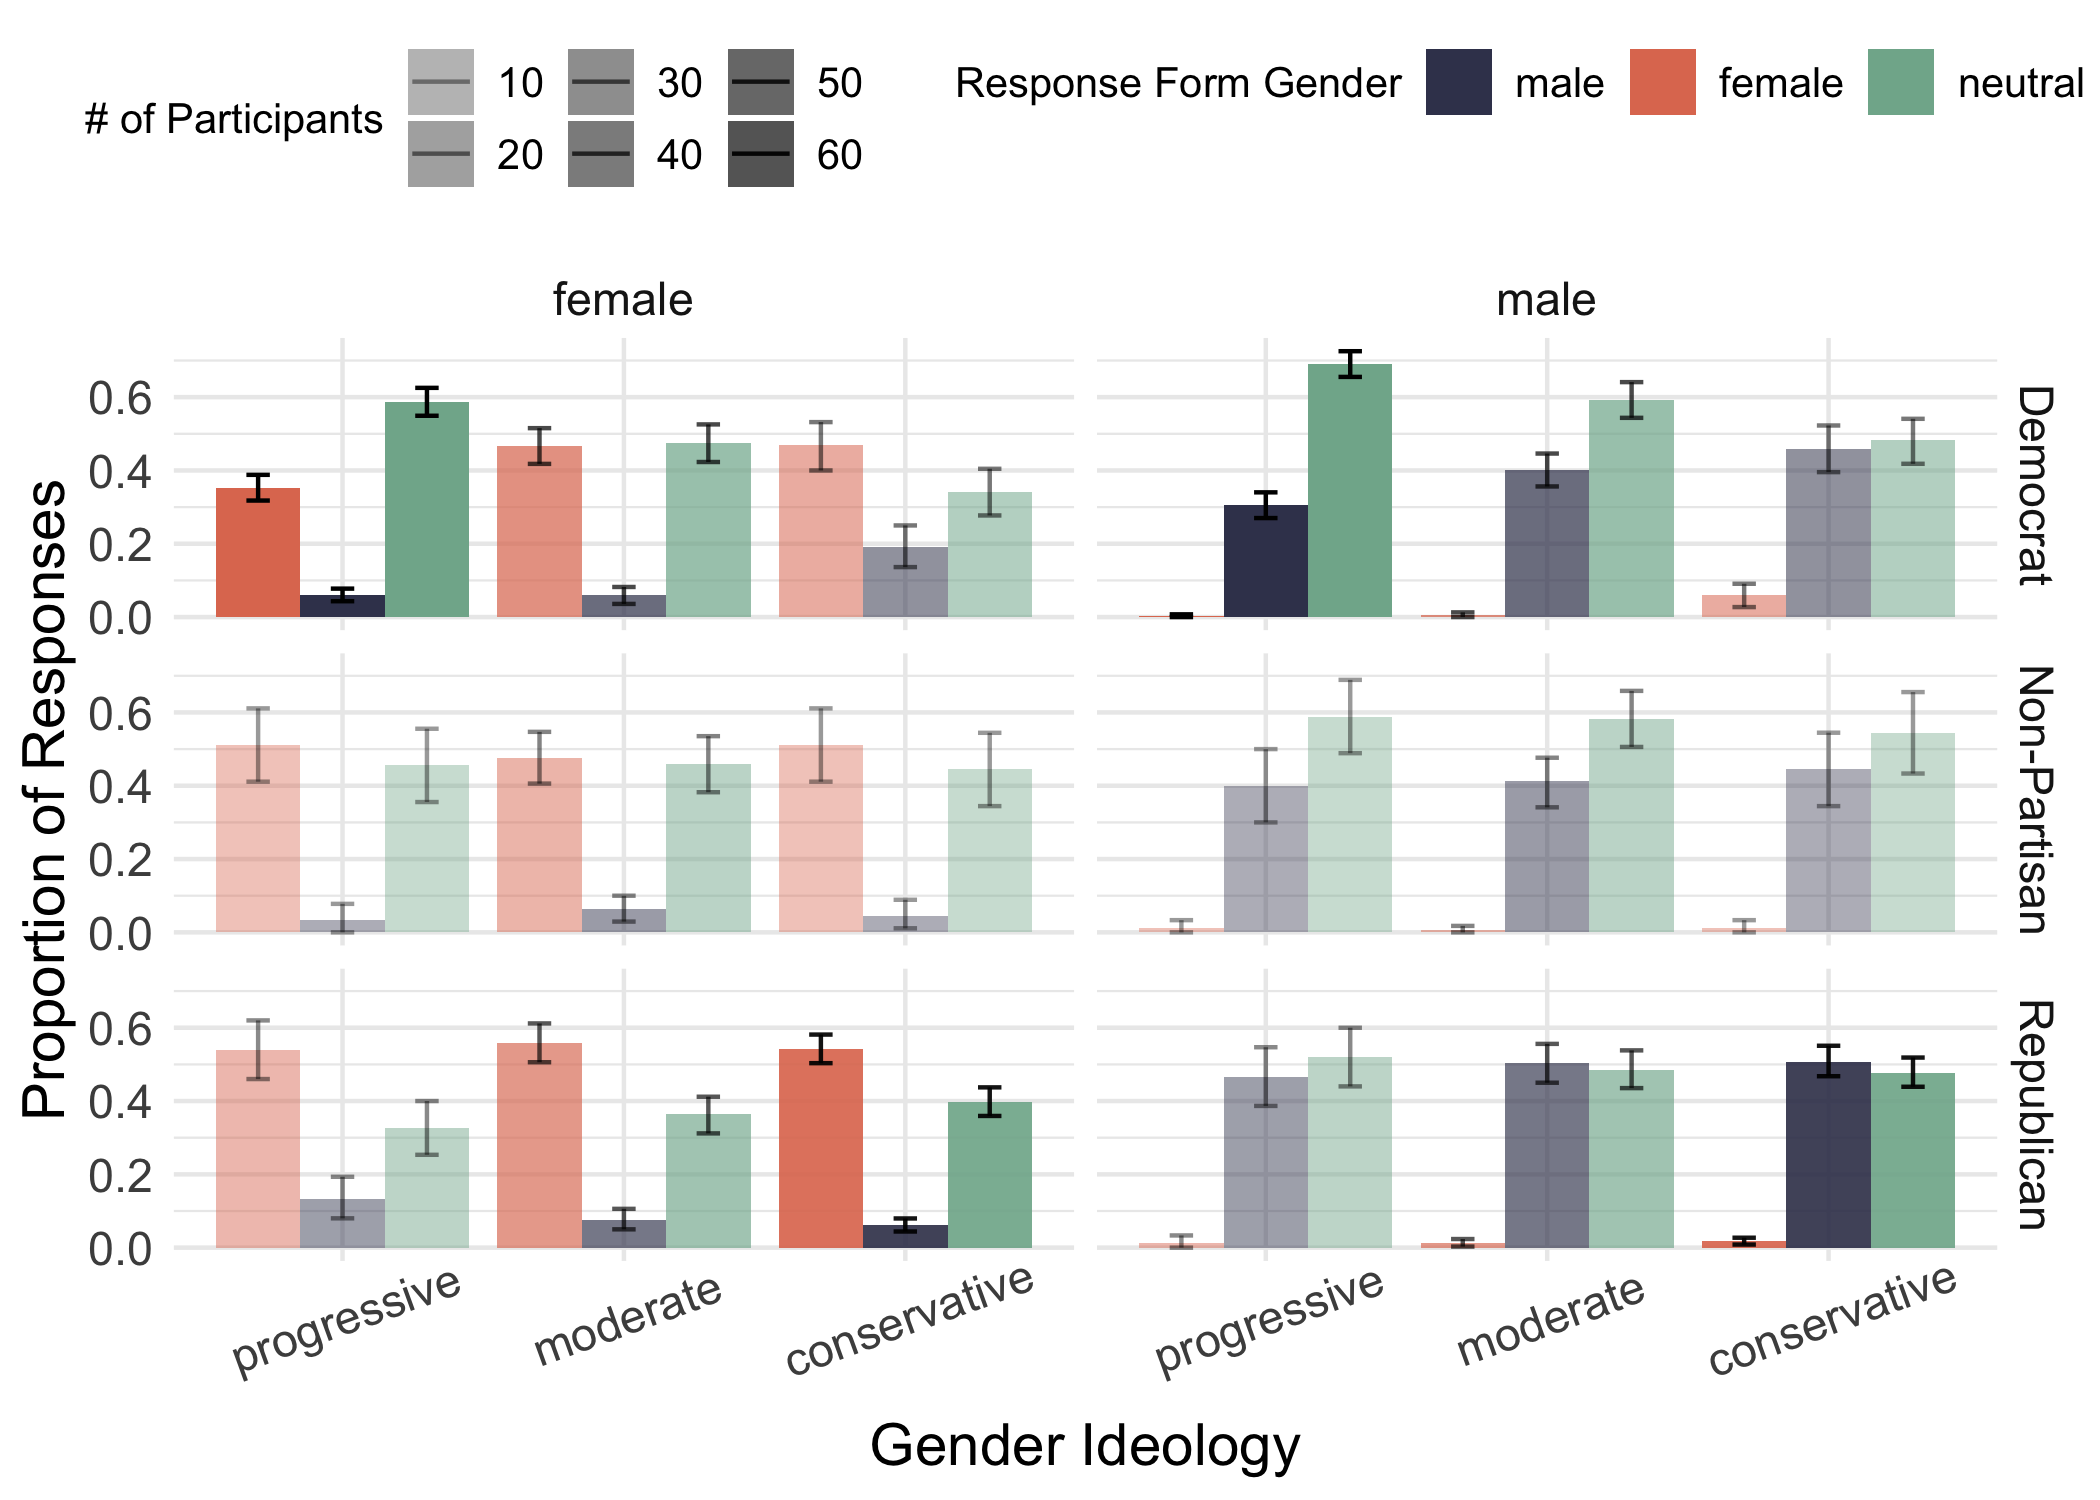
\includegraphics[scale=0.115]{prod-3x2x3.png}
		\caption{Proportion of responses by gender produced in Experiment Two, according to gender of the name in the stimulus sentence (x-axis facet) and participant political alignment (y-axis facet)}
	\end{figure}
	
	\section{General Discussion}
	
	\section{Acknowledgments}
	
	\section{Supplementary Material}
	Supplementary materials, including details related to the norming study and the unreported processing study, can be found at \textbf{ADD URL}.
	
	
	\printbibliography
	
	
	
\end{document}